\documentclass[xcolor=pdflatex,dvipsnames,table]{beamer}
\usepackage{epsfig,graphicx}
\usepackage{palatino}
\usepackage{fancybox}
\usepackage{relsize}
\usepackage[procnames]{listings}
\usepackage{hyperref}
\usepackage{qtree} % needed?
\usepackage{booktabs}
\usepackage{dirtree}
\usepackage[normalem]{ulem}


% fatter TT font
\renewcommand*\ttdefault{txtt}
% another TT, suggested by Alex
% \usepackage{inconsolata}
% \usepackage[T1]{fontenc} % needed as well?


\newcommand{\scale}{0.7}

\newcommand{\todo}[1]{{\emph{TODO: #1}}}
\newcommand{\martin}[1]{{\color{blue} Martin: #1}}
\newcommand{\abcdef}[1]{{\color{red} Author2: #1}}

% uncomment following for final submission
%\renewcommand{\todo}[1]{}
%\renewcommand{\martin}[1]{}
%\renewcommand{\author2}[1]{}

\newcommand{\code}[1]{{\texttt{#1}}}

\hypersetup{
  linkcolor  = black,
%  citecolor  = blue,
  urlcolor   = blue,
  colorlinks = true,
}

\beamertemplatenavigationsymbolsempty
\setbeamertemplate{footline}[frame number]





\newif\ifbook
% shared in slides and book

\lstdefinelanguage{chisel}{
  morekeywords={abstract,case,catch,class,def,%
    do,else,extends,false,final,finally,%
    for,if,implicit,import,match,mixin,%
    new,null,object,override,package,%
    private,protected,requires,return,sealed,%
    super,this,throw,trait,true,try,%
    type,val,var,while,with,yield},
  otherkeywords={=>,<-,<\%,<:,>:,\#,@},
  sensitive=true,
  morecomment=[l]{//},
  morecomment=[n]{/*}{*/},
  morestring=[b]",
  morestring=[b]',
  morestring=[b]"""
}

\usepackage{color}
\definecolor{dkgreen}{rgb}{0,0.6,0}
\definecolor{gray}{rgb}{0.5,0.5,0.5}
\definecolor{mauve}{rgb}{0.58,0,0.82}

% Default settings for code listings
\ifbook
\lstset{%frame=lines,
  language=chisel,
  aboveskip=3mm,
  belowskip=3mm,
  showstringspaces=false,
  columns=fixed, % basewidth=\mybasewidth,
  basicstyle={\small\ttfamily},
  numbers=none,
  numberstyle=\footnotesize,
  % identifierstyle=\color{red},
  breaklines=true,
  breakatwhitespace=true,
  procnamekeys={def, val, var, class, trait, object, extends},
  % procnamestyle=\ttfamily,
  tabsize=2,
  float
}
\else
\lstset{%frame=lines,
  language=chisel,
  aboveskip=3mm,
  belowskip=3mm,
  showstringspaces=false,
  columns=fixed, % basewidth=\mybasewidth,
  basicstyle={\small\ttfamily},
  numbers=none,
  numberstyle=\footnotesize\color{gray},
  % identifierstyle=\color{red},
  keywordstyle=\color{blue},
  commentstyle=\color{dkgreen},
  stringstyle=\color{mauve},
  breaklines=true,
  breakatwhitespace=true,
  procnamekeys={def, val, var, class, trait, object, extends},
  procnamestyle=\ttfamily\color{red},
  tabsize=2,
  float
}
\fi

\lstnewenvironment{chisel}[1][]
{\lstset{language=chisel,#1}}
{}

\newcommand{\shortlist}[1]{{\lstinputlisting[nolol]{#1}}}

\newcommand{\longlist}[3]{{\lstinputlisting[float, caption={#2}, label={#3}, frame=tb, captionpos=b]{#1}}}

\newcommand{\verylonglist}[3]{{\lstinputlisting[caption={#2}, label={#3}, frame=tb, captionpos=b]{#1}}}



\title{Components and Sequential Circuits}
\author{Martin Schoeberl}
\date{\today}
\institute{Technical University of Denmark\\
Embedded Systems Engineering}

\begin{document}

\begin{frame}
\titlepage
\end{frame}

\begin{frame}[fragile]{Overview}
\begin{itemize}
\item Vending machine project
\item Repeat combinational building blocks
\item Power user II
\item Components and top-level
\item Sequential circuits
%\item Chisel/VHLD comparison
\end{itemize}
\end{frame}


\begin{frame}[fragile]{Admin}
\begin{itemize}
\item How is the lab work going so far?
\item Start to organize yourself in groups of 2--3
\begin{itemize}
\item You can ask for finding a group via slack
\end{itemize}
\item Register at \href{https://docs.google.com/spreadsheets/d/1Hp81EyFYYvjm336DrwtCym9oRQUEzRKe6VceFp0ZCAQ/edit?usp=sharing}{Google spreadsheet}
\end{itemize}
\end{frame}


\begin{frame}[fragile]{A Vending Machine from 1952}
\begin{figure}
    \centering
    \href{https://en.wikipedia.org/wiki/File:CandiesVendingMachine1952.jpg}{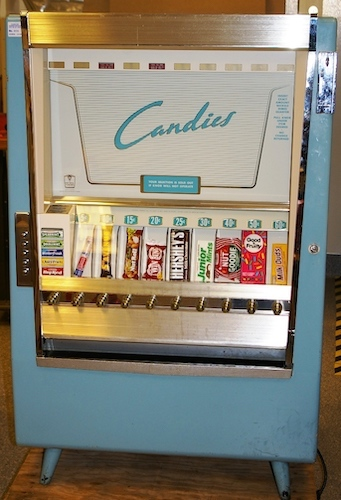
\includegraphics[scale=0.4]{CandiesVendingMachine1952}}

\end{figure}

{\tiny Source: Minnesota Historical Society, \href{https://creativecommons.org/licenses/by-sa/2.0}{CC BY-SA 2.0}}
\end{frame}

\begin{frame}[fragile]{The Vending Machine}
\begin{itemize}
\item Final project is a vending machine
\item \emph{Specification document is in DTU Inside (show it)}
\item Inputs: coins, buy
\item Display: price and current amount
\item Output: release can or error
\item Small challenge to multiplex the display
\item State machine with data path is the \emph{brain} of the VM
\item Guided step by step over several weeks
\end{itemize}
\end{frame}

\begin{frame}[fragile]{Vending Machine Specification I}
\begin{itemize}
\item Sell 1 item and not returning any money
\item Set price with 5 switches (1--31 kr.)
\item Display price on two 7-segment displays (hex.)
\item Accept 2 ad 5 kr. (two push buttons)
\item Display sum on two 7-segment displays (hex.)
\begin{itemize}
\item Amount entered so far
\end{itemize}
\item Does not return money, left for the next purchase
\end{itemize}
\end{frame}

\begin{frame}[fragile]{Vending Machine Specification II}
\begin{itemize}
\item Push button \emph{Buy}
\begin{itemize}
\item If not enough money, activate \emph{alarm} as long as buy is pressed
\item If enough money, activate \emph{release item} for as long as \emph{buy}
is pressed and reduce \emph{sum} by the price of the item
\end{itemize}
\item Optional extras (for a 12)
\begin{itemize}
\item Display decimal numbers
\item Supplement alarm by some visuals (e.g., blinking display)
\item Count coins and display an alarm when compartment is full ($>$ 20 coins)
\item Have some text scrolling on the display
\item ...
\item Your ideas :-)
\end{itemize}
\end{itemize}
\end{frame}

\begin{frame}[fragile]{Design and Implementation}
\begin{itemize}
\item Implementation shall be a state machine plus datapath
\item Design your datapath on a sheet of paper
\item Datapath
\begin{itemize}
\item Does add and subtract
\item Contains a register to hold the sum
\item Needs some mulitplexer to operate
\end{itemize}
\item Display needs multiplexing
\begin{itemize}
\item Implemented with some counters and a multiplexer
\end{itemize}
\item Show each part of your design to a TA
\begin{itemize}
\item 7-segment decoder, 7-segment with a counter, display multiplexer, complete vending machine
\end{itemize}
\end{itemize}
\end{frame}

\begin{frame}[fragile]{Vending Machine Design and Implementation Steps}
\begin{itemize}
\item We start next week
\item 2 + 2 + 3 + 3 + 4 + 4 = 18 supervised lab hours
\item 1a. Hexadecimal to 7-segment decoder
\item 1b. 7-segment display with a counter
\item 2. Multiplexed Seven-Segment Display
\item 3. Complete Vending Machine
\item \emph{Show your working design to a TA}
\end{itemize}
\end{frame}

\begin{frame}[fragile]{Final Report}
\begin{itemize}
\item One report per group
\item A single PDF
\begin{itemize}
\item Your group number is part of the file name (e.g., group7.pdf)
\item Code as listing in an appendix (no .zip files)
\item Hand in in DTU Inside
\end{itemize}
\item Content
\begin{itemize}
\item Abstract
\item Preface (Who did what)
\end{itemize}
\begin{enumerate}
\item Introduction and Problem Formulation
\item Analysis and Design
\item Implementation
\item Testing
\item Results
\item Discussion
\item Conclusion
\end{enumerate}
\begin{itemize}
\item List of References
\item Appendix: Chisel code
\end{itemize}
\end{itemize}
\end{frame}

\begin{frame}[fragile]{Questions on Final Project?}
\end{frame}

\begin{frame}[fragile]{Combinational Circuit with Conditional Update}
\begin{itemize}
\item Value first needs to be wrapped into a \code{Wire}
\item Updates with the Chisel update operation \code{:=}
\item With \code{when} we can express a conditional update
\item The condition is an expression with a Boolean result
\item The resulting circuit is a multiplexer
\item The rule is that the last enabled assignment counts
\begin{itemize}
\item Here the order of statements has a meaning
\end{itemize}
\end{itemize}
\shortlist{../code/comb_wire2.txt}
\end{frame}

\begin{frame}[fragile]{Comparison}
\begin{itemize}
\item The usual operations (as in Java or C)
\begin{itemize}
\item Unusual equal and unequal operator symbols
\item To keep the original Sala operators usable for references
\end{itemize}
\item Operands are \code{UInt} and \code{SInt}
\item Operands can be \code{Bool} for equal and unequal
\item Result is \code{Bool}
\end{itemize}
\begin{chisel}
>, >=, <, <=
===, =/=
\end{chisel}
\end{frame}

\begin{frame}[fragile]{Boolean Logical Operations}
\begin{itemize}
\item Operands and result are \code{Bool}
\item Logical NOT, AND, and OR
\end{itemize}
\begin{chisel}
val notX = !x
val bothTrue = a && b
val orVal = x || y
\end{chisel}
\end{frame}

\begin{frame}[fragile]{The ``Else'' Branch}
\begin{itemize}
\item We can express a form of ``else''
\item Note the \code{.} in \code{.otherwise}
\end{itemize}
\shortlist{../code/comb_otherwise.txt}
\end{frame}



\begin{frame}[fragile]{A Chain of Conditions}
\begin{itemize}
\item To test for different conditions
\item Select with a priority order
\item The first expression that is true counts
\item The hardware is a chain of multiplexers
\end{itemize}
\begin{columns}
\column{0.5\textwidth}
\shortlist{../code/comb_elsewhen.txt}
\column{0.5\textwidth}
\begin{figure}
  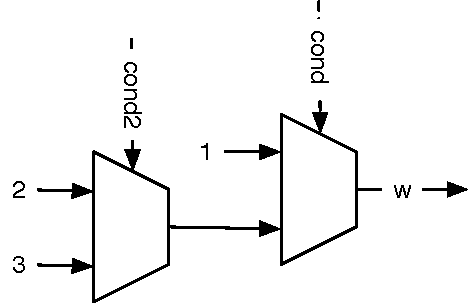
\includegraphics[scale=\scale]{../figures/mux-chain}
\end{figure}
\end{columns}
\end{frame}

\begin{frame}[fragile]{Default Assignment}
\begin{itemize}
\item Practical for complex expressions
\item Forgetting to assign a value on all conditions
\begin{itemize}
\item Would describe a latch
\item Runtime error in Chisel
\end{itemize}
\item Assign a default value is good practise
\end{itemize}
\shortlist{../code/comb_wiredefault.txt}
\end{frame}

\begin{frame}[fragile]{Logic Can Be Expressed as a Table}
\begin{itemize}
\item Sometimes more convenient 
\item Still combinational logic (gates)
\item Is converted to Boolean expressions
\item Let the synthesize tool do the conversion!
\item We use the \code{switch} statement
\end{itemize}
\shortlist{../code/encdec_decbin.txt}
\end{frame}


\begin{frame}[fragile]{A Decoder}
\begin{figure}
  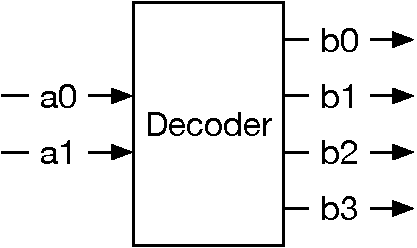
\includegraphics[scale=\scale]{../figures/decoder}
\end{figure}
\begin{itemize}
\item Converts a binary number of $n$ bits to an $m$-bit signal, where $m \leq 2^n$
\item The output is one-hot encoded (exactly one bit is one)
\item Building block for a $m$-way Mux
\item Used for address decoding in a computer system
\item Maybe of use for the display multiplexer
\end{itemize}
\end{frame}

\begin{frame}[fragile]{Truth Table of a Decoder}
\begin{table}
  \begin{tabular}{rr}
    \toprule
    a & b \\
    \midrule
    00 & 0001 \\
    01 & 0010 \\
    10 & 0100 \\
    11 & 1000 \\
    \bottomrule 
  \end{tabular} 
\end{table}
\end{frame}

\begin{frame}[fragile]{An Encoder}
\begin{figure}
  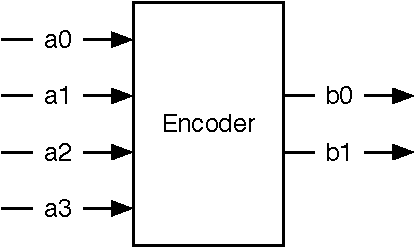
\includegraphics[scale=\scale]{../figures/encoder}
\end{figure}
\begin{itemize}
\item Converts one-hot encoded signal
\item To binary representation
\end{itemize}
\end{frame}

\begin{frame}[fragile]{Truth Table of an Encoder}
\begin{table}
  \begin{tabular}{rr}
    \toprule
    a & b \\
    \midrule
    0001 & 00 \\
    0010 & 01 \\
    0100 & 10 \\
    1000 & 11 \\
    ???? & ?? \\
    \bottomrule 
  \end{tabular} 
\end{table}
\begin{itemize}
\item Only defined for one-hot input
\end{itemize}
\end{frame}

\begin{frame}[fragile]{Encoder in Chisel}
\begin{itemize}
\item We cannot describe a function with undefined outputs
\item We use a default assignment of \code{"b00"}
\end{itemize}
\shortlist{../code/encdec_enc.txt}
\end{frame}


\begin{frame}[fragile]{Power User II}
\begin{itemize}
\item Every craftsmen starts with good-quality tools
\item ``Tools amplify your talent''\footnote{The Pragmatic Programmer: From Journeyman to Master, by Andrew Hunt and David Thomas}
\begin{itemize}
\item The better your tools, the more productive you are
\item The better you know them, the more productive you are
\end{itemize}
\item IDEs (Eclipse, InelliJ) are nice, I love them too
\item But we shall go beyond it
\item Use tools (and write your own)
\item Help with: google, man pages, or even plain --help (or -h)
\item \url{https://www.oreilly.com/learning/ten-steps-to-linux-survival}
\begin{itemize}
\item This is about command line tools, not just Linux
\end{itemize}
\end{itemize}
\end{frame}

\begin{frame}[fragile]{Power User II}
\begin{itemize}
\item Use the command line, shell, terminal
\item In Windows: PowerShell
\begin{itemize}
\item You may want to install the Linux subsystem
\end{itemize}
\item Universal Unix commands (Windows, Mac, Linux)
\item Navigating the file system:
\begin{itemize}
\item Change directory: \code{cd}
\item Print working directory: \code{pwd}
\item Make a directory: \code{mkdir abc}
\item Create a file: \code{echo test > abc.txt}
\item Show file content: \code{cat abc.txt}
\item Remove a file: \code{rm abc.txt}
\end{itemize}
\item Run your Chisel code with \code{sbt run}
\item You used the terminal already from within IntelliJ ;-)
\end{itemize}
\end{frame}

\begin{frame}[fragile]{Power User II}
\begin{itemize}
\item We talked about \code{git} last week
\item To version your source
\item Maybe hosting on GitHub
\item Most teaching material is on GitHub
\item Use \code{git pull} to update the lab material
\item Show how to use it, now!
\begin{itemize}
\item Clone a repo: \code{git clone path}
\item Get the newest version: \code{git pull}
\item Further commands: \code{git commit, push, log, status}
\item Overview of changes: \code{gitk}
\end{itemize}
\end{itemize}
\end{frame}

\begin{frame}[fragile]{Structure With Bundles}
\begin{itemize}
\item A \code{Bundle} to group signals
\item Can be different types
\item Defined by a class that extends \code{Bundle}
\item Named fields as \code{val}s within the block
\item Like a C struct or VHDL record
\end{itemize}
\shortlist{../code/bundle.txt}
\end{frame}

\begin{frame}[fragile]{Using a Bundle}
\begin{itemize}
\item Create it with \code{new}
\item Wrap it into a \code{Wire}
\item Field access with \emph{dot} notation
\end{itemize}
\shortlist{../code/bundle_use.txt}
\end{frame}



\begin{frame}[fragile]{Components}
\begin{itemize}
\item Components are building blocks
\item The have input and output ports (= pins)
\begin{itemize}
\item Organized as a \code{Bundle}
\item assigned to field \code{io}
\end{itemize}
\item We build circuits as a hierarchy of components
\item In Chisel a component is called \code{Module}
\item Components/Modules are used to organize the circuit
\begin{itemize}
\item Similar as using methods in Java
\end{itemize}
\end{itemize}
\end{frame}

\begin{frame}[fragile]{Hierarchy of Components Example}
\begin{figure}
  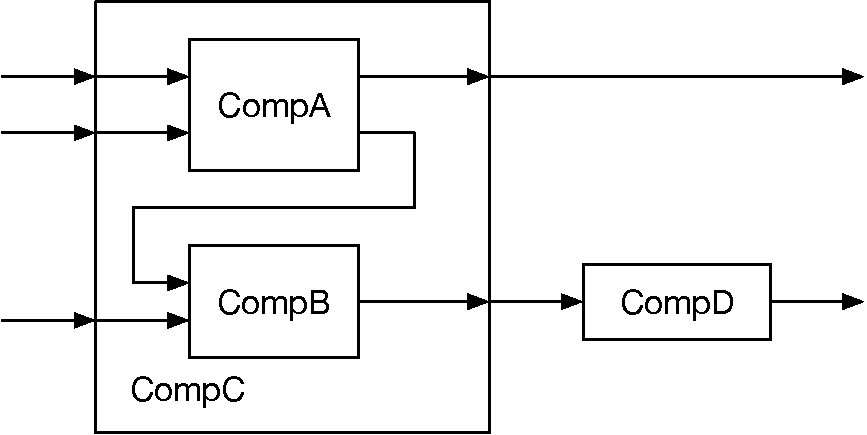
\includegraphics[scale=\scale]{../figures/components}
\end{figure}
\end{frame}


\begin{frame}[fragile]{Input/Output Ports}
\begin{itemize}
\item Ports are bundles with directions
\item Ports used to connect modules
\end{itemize}
\begin{chisel}
class AluIO extends Bundle {
  val function = Input(UInt(2.W))
  val inputA = Input(UInt(4.W))
  val inputB = Input(UInt(4.W))
  val result = Output(UInt(4.W))
}
\end{chisel}
\end{frame}


\begin{frame}[fragile]{An Adder Module}
\begin{itemize}
\item A \code{class} that \code{extends} \code{Module}
\item Interface (port) is a \code{Bundle}, wrapped into an \code{IO()}, and stored in the field \code{io}
\item Circuit description in the constructor
\end{itemize}
\begin{chisel}
class Adder extends Module {
  val io = IO(new Bundle {
    val a = Input(UInt(4.W))
    val b = Input(UInt(4.W))
    val result = Output(UInt(4.W))
  })

  val addVal = io.a + io.b
  io.result := addVal
}
\end{chisel}
\end{frame}

\begin{frame}[fragile]{Connections}
\begin{itemize}
\item Simple connections just with assignments, e.g.,
\begin{chisel}
  adder.io.a := ina
  adder.io.b := inb
\end{chisel}
\item Note the dot access to the field \code{io} and then the IO field
\end{itemize}
\end{frame}



\begin{frame}[fragile]{Module Usage}
\begin{itemize}
\item Create with \code{new} and wrap into a \code{Module()}
\item Interface port via the \code{io} field
\item Note the assignment operator \code{:=} on \code{io} fields
\end{itemize}
\begin{chisel}
  val adder = Module(new Adder())
  adder.io.a := ina
  adder.io.b := inb
  val result = adder.io.result
\end{chisel}
\end{frame}

\begin{frame}[fragile]{Example: Arithmetic Logic Unit}
\begin{figure}
  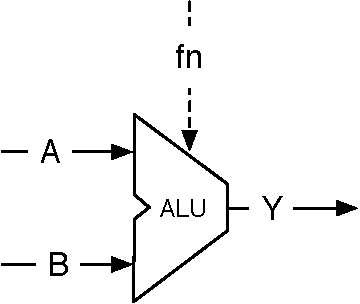
\includegraphics[scale=\scale]{../figures/alu}
\end{figure}
\begin{itemize}
\item Also called ALU
\item A central component of a microprocessor
\item Two inputs, one function select, and an output
\item Part of the \emph{datapath}
\end{itemize}
\end{frame}

\begin{frame}[fragile]{Example: Arithmetic Logic Unit}
\shortlist{../code/components_alu.txt}
\end{frame}

\begin{frame}[fragile]{Hierarchy of Components Example}
\begin{figure}
  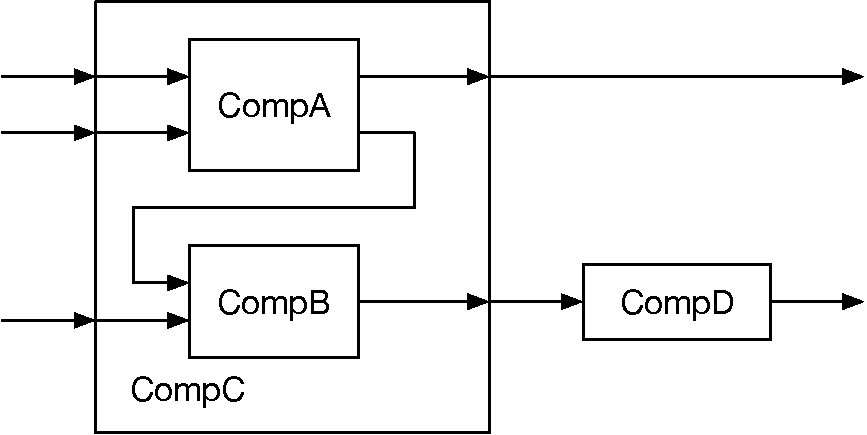
\includegraphics[scale=\scale]{../figures/components}
\end{figure}
\end{frame}

\begin{frame}[fragile]{Components CompA and CompB}
\shortlist{../code/components_ab.txt}
\end{frame}

\begin{frame}[fragile]{Component CompC}
\shortlist{../code/components_c.txt}
\end{frame}









\begin{frame}[fragile]{Chisel Main}

\begin{itemize}
\item Create one top-level Module
\item Invoke the Chisel driver from the App
\item Pass the top module (e.g., \code{new Hello()})
\item Optional: pass some parameters (in the \code{Array})
\item Following code generates Verilog code for \emph{Hello World}
\end{itemize}
\begin{chisel}
object Hello extends App {
  chisel3.Driver.execute(Array[String](), () => new Hello())
}
\end{chisel}
\end{frame}

\begin{frame}[fragile]{Hello World in Chisel}
\shortlist{../code/hello.txt}
\end{frame}



\begin{frame}[fragile]{Generated Verilog for Hello}
\begin{itemize}
\item \code{Hello} is the top-level of our blinking LED
\item No real need to read this code
\item But pin assignment for the synthsis
\item Additional pins: \code{clock} and \code{reset}
\item User pin names with a leading \code{io\_}
\end{itemize}
\begin{verbatim}
module Hello(
  input   clock,
  input   reset,
  output  io_led
);
\end{verbatim}
\end{frame}

\begin{frame}[fragile]{Generated Verilog for Hello}
\begin{itemize}
\item We can find our two register definitions
\item \code{@...} gives Chisel source and line number (e.g., 17)
\end{itemize}
\begin{verbatim}
  reg [31:0] cntReg; // @[Hello.scala 17:23]
  reg [31:0] _RAND_0;
  reg  blkReg; // @[Hello.scala 18:23]
\end{verbatim}
\end{frame}

\begin{frame}[fragile]{Generated Verilog for Hello}
\begin{itemize}
\item The increment and comparison against maximum value
\end{itemize}
\begin{verbatim}
  assign _T_1 = cntReg + 32'h1; // @[Hello.scala 20:20]
  assign _T_2 = cntReg == 32'h2faf07f; // @[Hello.scala 21:15]
  assign _T_3 = ~ blkReg; // @[Hello.scala 23:15]
  assign io_led = blkReg; // @[Hello.scala 25:10]
\end{verbatim}
\end{frame}

\begin{frame}[fragile]{Generated Verilog for Hello}
\begin{itemize}
\item Verilog register code
\end{itemize}
\begin{verbatim}
  always @(posedge clock) begin
    if (reset) begin
      cntReg <= 32'h0;
    end else if (_T_2) begin
      cntReg <= 32'h0;
    end else begin
      cntReg <= _T_1;
    end
  end
\end{verbatim}
\end{frame}

\begin{frame}[fragile]{Verilog Generation Summary}
\begin{itemize}
\item Verilog is generated for synthesis
\item We do not need to read it
\item Just pins are interesting
\item Additional clock and reset
\item Pin names with additional \code{io\_}
\end{itemize}
\end{frame}

\begin{frame}[fragile]{File Organization in Scala/Chisel}
\begin{itemize}
\item A Scala file can contain several classes (and objects)
\item For large classes use one file per class with the class name
\item Scala has packages, like Java
\item Use folders with the package names for file organization
\item \code{sbt} looks into current folder and \code{src/main/scala/}
\item Tests shall be in \code{src/test/scala/}
\end{itemize}
\end{frame}

\begin{frame}[fragile]{File Organization in Scala/Chisel}
\dirtree{%
.1 project.
.2 src.
.3 main.
.4 scala.
.5 package.
.6 sub-package.
.3 test.
.4 scala.
.5 package.
.2 target.
.2 generated.
}
\end{frame}

\begin{frame}[fragile]{What is a Minimal Chisel Project?}
\begin{itemize}
\item Scala class (e.g., \code{Hello.scala})
\item Build info in \code{build.sbt} for \code{sbt}:
\end{itemize}
\begin{chisel}
scalaVersion := "2.11.12"

libraryDependencies += "edu.berkeley.cs" %% "chisel3" % "3.2.2"
\end{chisel}
\end{frame}



\begin{frame}[fragile]{Sequential Building Blocks}
\begin{itemize}
\item Contain a register
\item Plus combinational circuits
\end{itemize}
\begin{figure}
  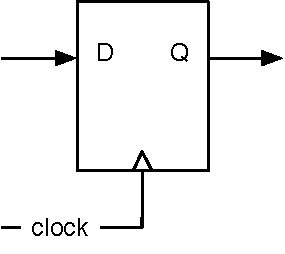
\includegraphics[scale=\scale]{../figures/register}
\end{figure}
\shortlist{../code/sequ_reg.txt}
\end{frame}

\begin{frame}[fragile]{Register With Reset}
\begin{figure}
  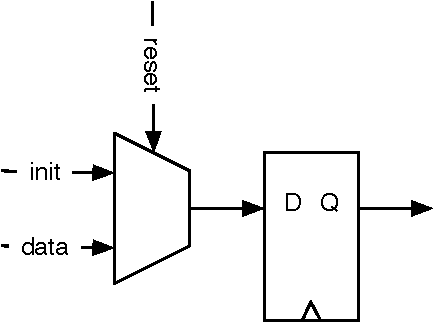
\includegraphics[scale=\scale]{../figures/register-reset}
\end{figure}
\shortlist{../code/sequ_reg_init.txt}
\end{frame}

\begin{frame}[fragile]{Timing Diagram of the Register with Reset}
\begin{figure}
  \includegraphics[scale=1]{../figures/reg_wave}
\end{figure}
\begin{itemize}
\item Also called waveform diagram
\item Logic function over time
\item Can be used to describe a circuit function
\item Useful for debugging
\end{itemize}
\end{frame}

\begin{frame}[fragile]{Register with Enable}
\begin{figure}
  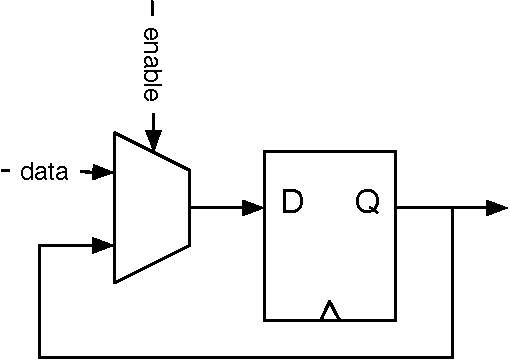
\includegraphics[scale=\scale]{../figures/register-enable}
\end{figure}
\begin{itemize}
\item Only when \code{enable} true is a value is stored
\end{itemize}
\shortlist{../code/sequ_reg_ena.txt}

\end{frame}

\begin{frame}[fragile]{A Register with Reset and Enable}
\begin{itemize}
\item We can combine initialization and enable
\end{itemize}
\shortlist{../code/sequ_reg_init_ena.txt}
\begin{itemize}
\item A register can also be part of an expression
\item What does the following circuit do?
\end{itemize}
\shortlist{../code/sequ_reg_rising.txt}
\end{frame}


\begin{frame}[fragile]{A Register with an Adder is a Counter}
\begin{figure}
  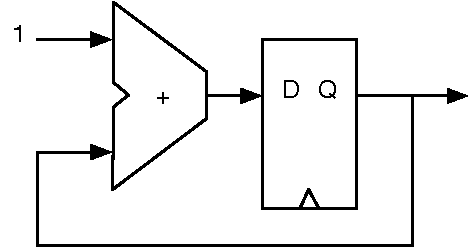
\includegraphics[scale=\scale]{../figures/counter}
\end{figure}
\begin{itemize}
\item Is a free running counter
\item 0, 1, ... 14, 15, 0, 1, ...
\end{itemize}
\shortlist{../code/sequ_free_counter.txt}
\end{frame}


\begin{frame}[fragile]{A Counter with a Mux}
\shortlist{../code/counter.txt}
\begin{itemize}
\item This counter counts from 0 to 9
\item And starts from 0 again after reaching 9
\begin{itemize}
\item Starting from 0 is common in computer engineering
\end{itemize}
\item A counter is the hardware version of a \emph{for loop}
\item Often needed
\end{itemize}
\end{frame}

\begin{frame}[fragile]{Counting Events}
\begin{figure}
  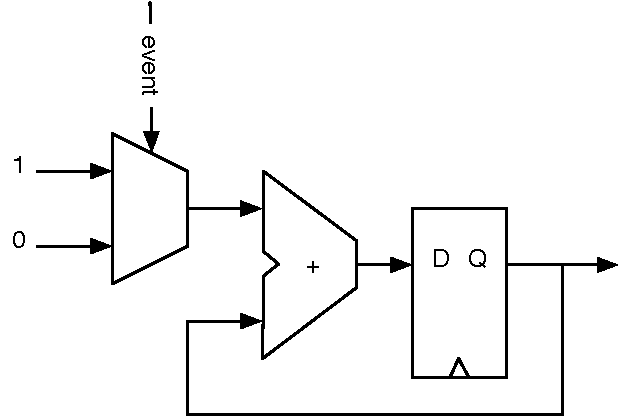
\includegraphics[scale=\scale]{../figures/event-counter}
\end{figure}
\shortlist{../code/sequ_event_counter.txt}
\end{frame}


\begin{frame}[fragile]{Counting Up and Down}
\begin{itemize}
\item Up:
\shortlist{../code/when_counter.txt}
\item Down:
\shortlist{../code/down_counter.txt}
\end{itemize}
\end{frame}



\begin{frame}[fragile]{Generating Timing with Counters}
\begin{itemize}
\item Generate a \code{tick} at a lower frequency
\item E.g., used for driving the display multiplexing at 1~kHz
\end{itemize}
\begin{figure}
  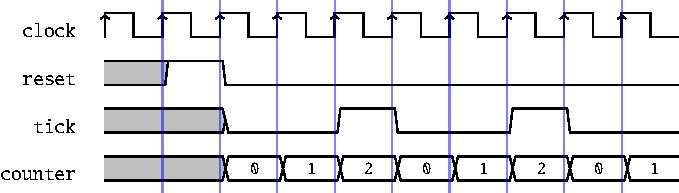
\includegraphics[scale=0.8]{../figures/tick_wave}
\end{figure}
\end{frame}


\begin{frame}[fragile]{The Tick Generation}
\shortlist{../code/sequ_tick_gen.txt}
\end{frame}

\begin{frame}[fragile]{Using the Tick}
\begin{itemize}
\item A counter running at a \emph{slower frequency}
\item By using the \code{tick} as an enable signal
\end{itemize}
\shortlist{../code/sequ_tick_counter.txt}
\end{frame}

\begin{frame}[fragile]{The \emph{Slow} Counter}
\begin{itemize}
\item Increment every \code{tick}
\end{itemize}
\begin{figure}
  \includegraphics[scale=0.8]{../figures/tick_count_wave}
\end{figure}
\end{frame}

\begin{frame}[fragile]{A Timer}
\begin{itemize}
\item Like a kitchen timer
\item Start by loading with a value
\item Count down till 0
\item Assert \code{done} when finished
\end{itemize}
\end{frame}

\begin{frame}[fragile]{One-Shot Timer}
\begin{figure}
  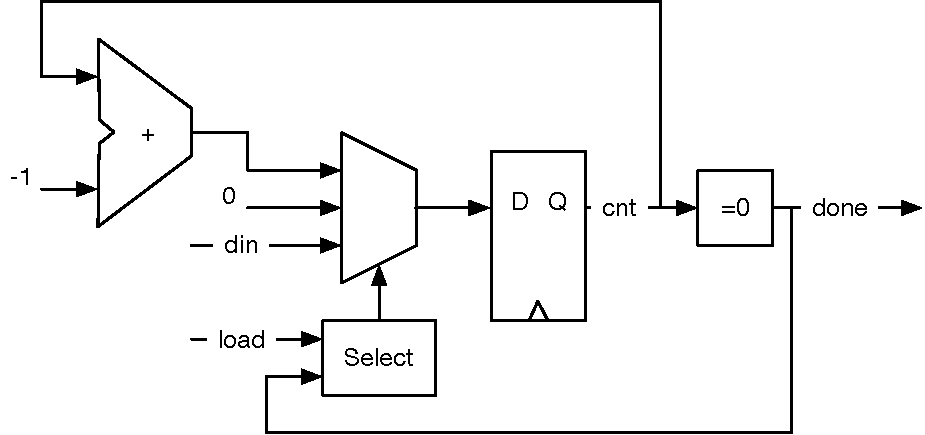
\includegraphics[scale=\scale]{../figures/timer}
\end{figure}
\end{frame}

\begin{frame}[fragile]{One-Shot Timer}
\shortlist{../code/timer.txt}
\end{frame}

\begin{frame}[fragile]{Summary on Counters}
\begin{itemize}
\item Counters are versatile tools
\item Count events
\item Generate timing ticks
\item Generate a one-shot timer
\end{itemize}
\end{frame}


\begin{frame}[fragile]{Preview: Testing with Chisel}
\begin{itemize}
\item Tester extends class \code{PeekPokeTester}
\item Has the device under test (DUT) as parameter
\item Testing code can use all features of Scala
\end{itemize}
\begin{chisel}
class CounterTester(dut: Counter) extends PeekPokeTester(dut) {

  // Here comes the Chisel/Scala code
  // for the testing
}
\end{chisel}
\end{frame}

\begin{frame}[fragile]{Testing}
\begin{itemize}
\item Set input values with \code{poke}
\item Advance the simulation with \code{step}
\item Read the output values with \code{peek}
\item Compare the values with \code{expect}
\end{itemize}
\end{frame}

\begin{frame}[fragile]{Testing Example}
\begin{chisel}
// Set input values
poke(dut.io.a, 3)
poke(dut.io.b, 4)
// Execute one iteration
step(1)
// Print the result
val res = peek(dut.io.result)
println(res)

// Or compare against expected value
expect(dut.io.result, 7)
\end{chisel}
\end{frame}

\begin{frame}[fragile]{Chisel Main for Testing}
\begin{itemize}
\item Tests can be written in Scala/Chisel
\item Invoke \code{execute} with some parameters, the DUT, and a tester
\end{itemize}
\begin{chisel}
object CounterTester extends App {

  iotesters.Driver.execute(Array[String](), () => new Counter(2)) {
    c => new CounterTester(c)
  }
}
\end{chisel}
\begin{itemize}
\item More on testing and waveform generation next week
\end{itemize}
\end{frame}


\begin{frame}[fragile]{Common Acronyms}
\begin{description}
\item [ADC] analog-to-digital converter
\item [ALU] arithmetic and logic unit
\item [ASIC] application-specific integrated circuit
\item [Chisel] constructing hardware in a Scala embedded language
\item [CISC] complex instruction set computer
\item [CRC] cyclic redundancy check
\item [DFF] D flip-flop, data flip-flop
\item [DMA] direct memory access
\item [DRAM] dynamic random access memory
\item [FF] flip-flop
\item [FIFO] first-in, first-out
\item [FPGA] field-programmable gate array
\item [HDL] hardware description language
\item [HLS] high-level synthesis
\item [IC] instruction count
\item [IDE] integrated development environment
\item [IO] input/output
\end{description}
\end{frame}

\begin{frame}[fragile]{Common Acronyms II}
\begin{description}
\item [ISA] instruction set architecture
\item [JDK] Java development kit
\item [JIT] just-Iin-time
\item [JVM] Java virtual machine
\item [LC] logic cell
\item [LRU] least-recently used
\item [MMIO] memory-mapped IO
\item [MUX] multiplexer
\item [OO] object oriented
\item [RISC] reduced instruction set computer
\item [SDRAM] synchronous DRAM
\item [SRAM] static random access memory
\item [TOS] top-of stack
\item [UART] universal asynchronous receiver/transmitter
\item [VHDL] VHSIC hardware description language
\item [VHSIC] very high speed integrated circuit
\end{description}
\end{frame}


\begin{frame}[fragile]{Lab Today}
\begin{itemize}
\item Components and Small Sequential Circuits
\item \href{https://github.com/schoeberl/chisel-lab/tree/master/lab4}{Lab 4 Page}
\item You need to download again, as I have updated the lab
\begin{itemize}
\item Or learn to use git and do a  \code{git pull} ;-)
\end{itemize}
\item Each exercise contains a test, which initially fails
\item \code{sbt test} runs them all
\begin{itemize}
\item To just run a single test, run e.g.,\\
\code{sbt "testOnly SingleTest"}
\end{itemize}
When all test succeed your are done ;-)
\item Except: additional some drawing exercise
\end{itemize}
\end{frame}

\begin{frame}[fragile]{Summary}
\begin{itemize}
\item Vending machine is your final project
\item The vending machine and the report are part of your grade
\item A digital circuit is organized in components
\item Components have ports with directions
\item Sequential circuits are combinations of registers with combinational circuits
\end{itemize}
\end{frame}

\end{document}